\pagebreak
\section{Motor Tests}
\nopagebreak
\subsection{Armature Resistance} %\label{put a label here and uncomment}
\textbf{Name: Group 510}\\
\textbf{Date: 30/09 - 2015}

\subsubsection{Purpose}
The purpose of the test is to measure the armature resistance $R_a$.

\subsubsection{Setup}
\begin{figure}[H]
  \centering
	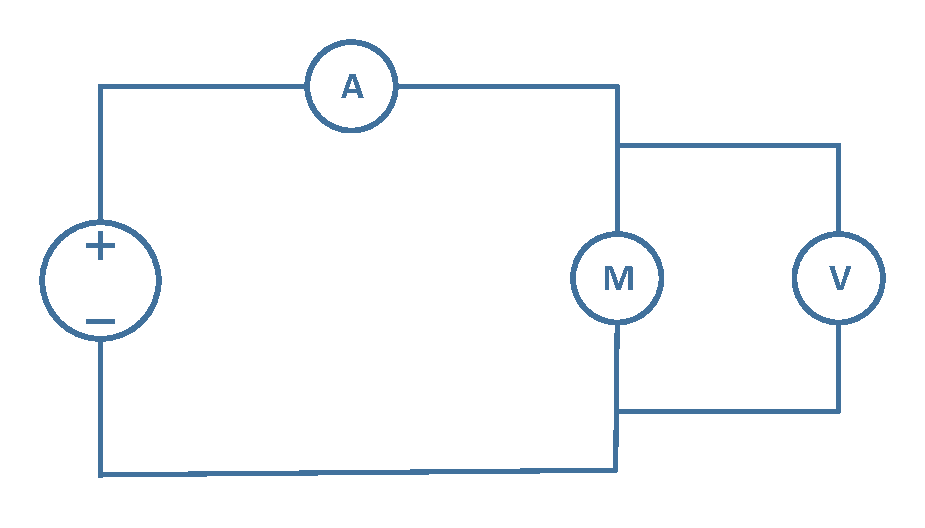
\includegraphics[scale=0.5]{figures/MotorTest1.pdf}
	\caption{Setup diagram}
\end{figure}

\subsubsection{List of Equipment}
Example of list of equipment:
\begin{table}[H]
\begin{tabular}{|l|l|p{4cm}|}
\hline%------------------------------------------------------------------------------------
  \textbf{Instrument}                        &  \textbf{AAU-no.}  &  \textbf{Type}       \\
\hline%------------------------------------------------------------------------------------
  Multimeter 1                               &  60764             &  Fluke 189 True RMS  \\
\hline%------------------------------------------------------------------------------------
  Multimeter 2                   		         &  60769             &  Fluke 189 True RMS  \\
\hline%------------------------------------------------------------------------------------
  Power Supply \small{(0 - 32 V) (0 - 10 A)} &  77076             &  Ea - ps 7032 - 100  \\
\hline%------------------------------------------------------------------------------------
  Clamp for fixing the motor                 &  03039             &                      \\
\hline%------------------------------------------------------------------------------------
\end{tabular}
\end{table}

\subsubsection{Procedure}

\begin{enumerate}
  \item Turn on the two multimeters and choose Voltage and Ampere settings respectively.
  \item Fix the motor shaft so it does not turn.
  \item Choose the first current value ($0.5$ A) on the current limiting of the power supply.
  \item Turn on the power supply and adjust the current limiting in accordance with the ampere meter.
  \item Repeat the two previous steps for each measurement of $0.5$ A increments up to $5$ A.
  \item Switch the poles of the power supply and repeat the measurements in the negative direction.
\end{enumerate}

\subsubsection{Results}

\begin{table}[H]
\begin{tabular}{|l|l|l| l|l|}
\cline{1-2}\cline{4-5}%-----------------------             ----------------------------------------------
  \textbf{Input (A)}   & \textbf{Output (V)} &\phantom{hey}& \textbf{Input (A)}   & \textbf{Output (V)}\\
\cline{1-2}\cline{4-5}%-----------------------             ----------------------------------------------
  $-5.0$               &            $-0.71$  &             & $0.5$                & $0.16$             \\
\cline{1-2}\cline{4-5}%-----------------------             ----------------------------------------------
  $-4.5$               &            $-0.65$  &             & $1.0$                & $0.34$             \\
\cline{1-2}\cline{4-5}%-----------------------             ----------------------------------------------
  $-4.0$               &            $-0.59$  &             & $1.5$                & $0.53$             \\
\cline{1-2}\cline{4-5}%-----------------------             ----------------------------------------------
  $-3.5$               &            $-0.54$  &             & $2.0$                & $0.62$             \\
\cline{1-2}\cline{4-5}%-----------------------             ----------------------------------------------
  $-3.0$               &            $-0.43$  &             & $2.5$                & $0.64$             \\
\cline{1-2}\cline{4-5}%-----------------------             ----------------------------------------------
  $-2.5$               &            $-0.36$  &             & $3.0$                & $0.75$             \\
\cline{1-2}\cline{4-5}%-----------------------             ----------------------------------------------
  $-2.0$               &            $-0.27$  &             & $3.5$                & $0.78$             \\
\cline{1-2}\cline{4-5}%-----------------------             ----------------------------------------------
  $-1.5$               &            $-0.20$  &             & $4.0$                & $0.80$             \\
\cline{1-2}\cline{4-5}%-----------------------             ----------------------------------------------
  $-1.0$               &            $-0.14$  &             & $4.5$                & $0.83$             \\
\cline{1-2}\cline{4-5}%-----------------------             ----------------------------------------------
  $-0.5$               &            $-0.07$  &             & $5.0$                & $0.88$             \\
\cline{1-2}\cline{4-5}%-----------------------             ----------------------------------------------
\end{tabular}
\end{table}

\begin{figure}[H]
  \centering
 	%Trim margins @:   left        bottom       right       top
 	\adjustbox{ trim = {.15\width} {.30\height} {.15\width} {.30\height}, clip }
  {
    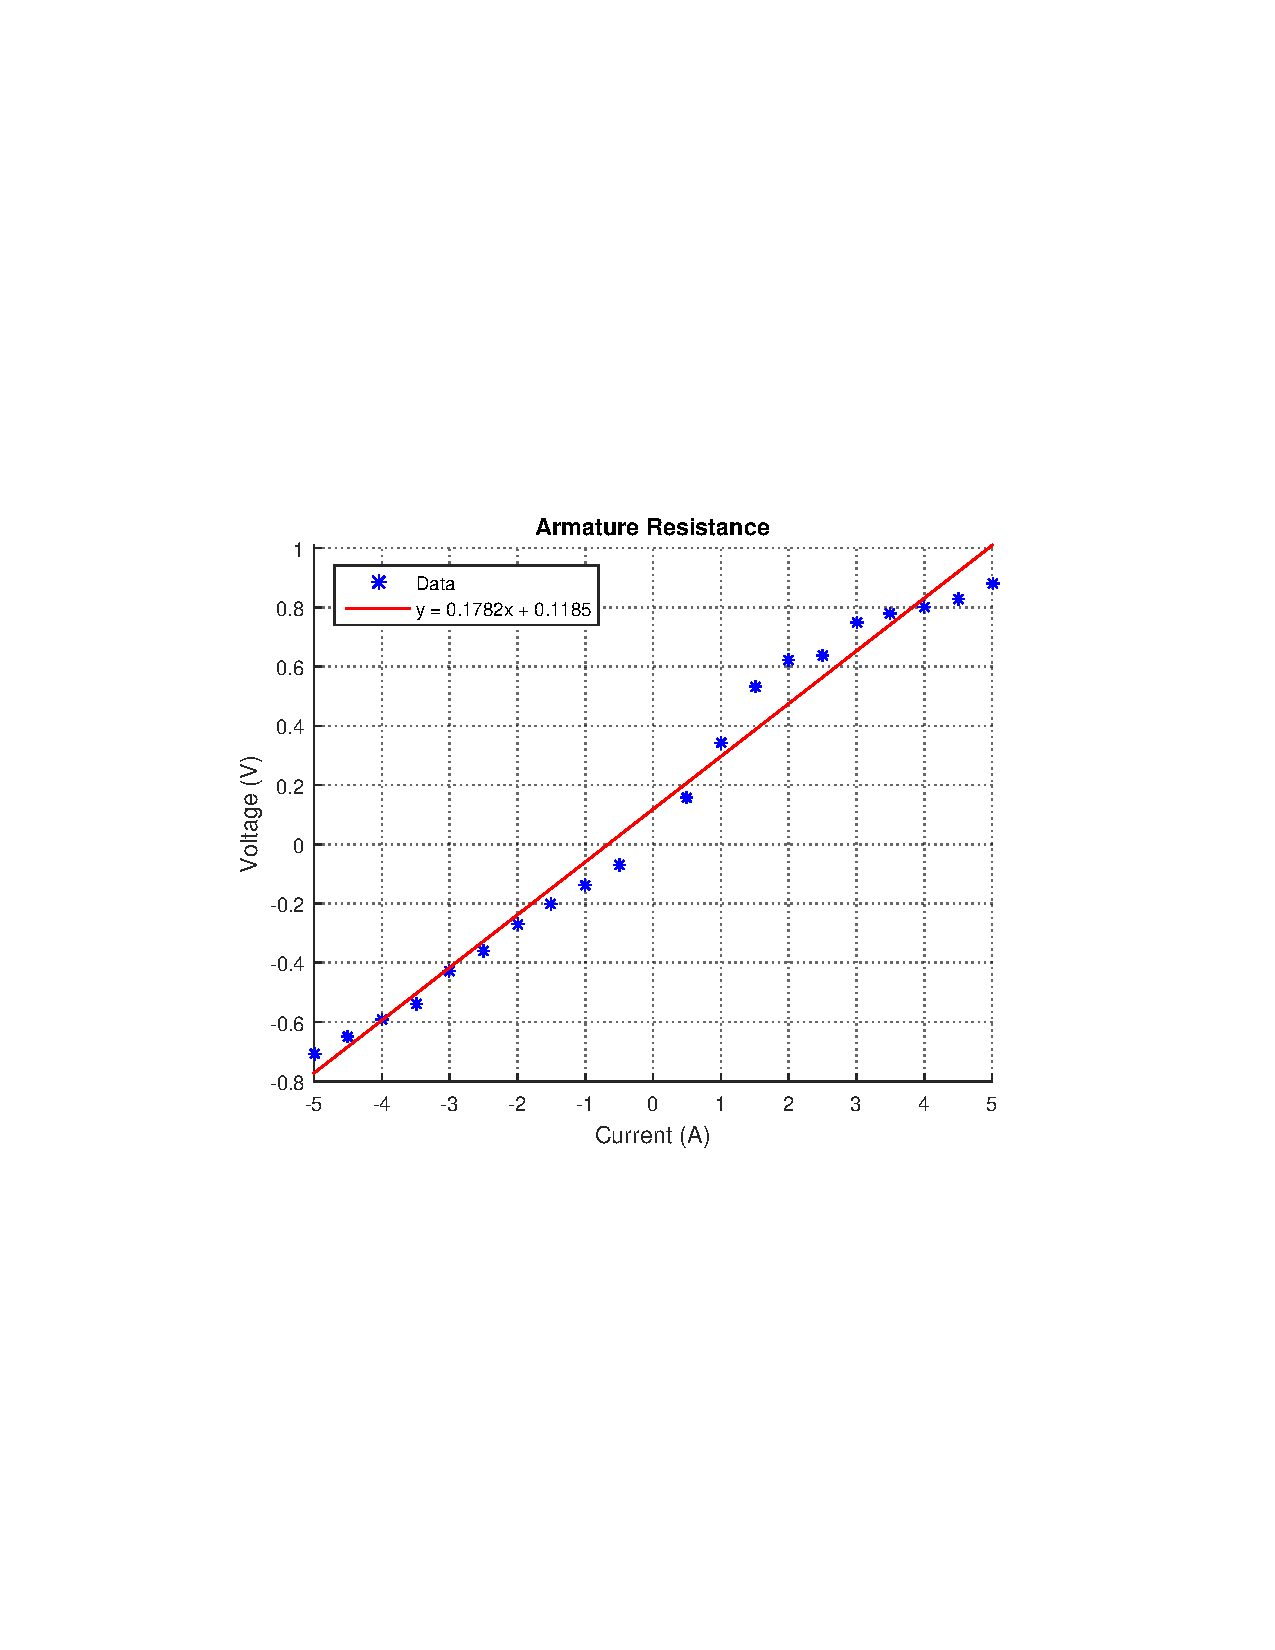
\includegraphics[width=\textwidth]{figures/armatureResistance.pdf}
  }
  \caption{Plot of test results}
  \label{armatureResistance}
\end{figure}

During these measurements the motor is in steady state. This is necessary for the inductor in the armature coil to act as a short circuit, which allows easy calculation of the armature resistance. In steady state we get:

\begin{flalign}
  I_a &= \frac{U_a}{R_a} \unit{A}\nonumber\\
  R_a &= \frac{U_a}{I_a} \unit{\Omega}\nonumber
\end{flalign}
\hspace{6mm} Where:\\
\begin{tabular}{p{1cm}ll}
  & $I_a$ & is the armature current     \\
  & $U_a$ & is the armature voltage     \\
  & $R_a$ & is the armature resistance  \\
\end{tabular}

As seen on the data plot in \figref{armatureResistance} we get a relatively linear function. The armature resistance is then approximated directly as the slope of the least square line, so we get:
$R_a = 0.178 \Omega$.